\documentclass{hippoidC}

\memoto{Idris}
\memosubject{Book of Proof}
\memodate{2024.03.11}
\status{\S 3.5 Binomial Theorem}

\begin{document}

\toc
\pagebreak

\begin{prooflist}{1. Write out Row 11 of Pascal’s triangle.}
    \item The first 6 terms of row 11 are unique, and the next fiver terms are mirrors of
        the first five.
    \item The terms of row 11 can be calculated with $\dbinom{11}{i}$, where $i
        \in \mathbb{N}, 0 \leq i \leq 11$.
    \item The $1^{st}$ and $11^{th}$ term of row 11 is
        $\dbinom{11}{0}=\dfrac{11!}{11!\cdot0!}=1$.
    \item The $2^{st}$ and $10^{th}$ term of row 11 is
        $\dbinom{11}{1}=\dfrac{11!}{10!\cdot1!}=11$.
    \item The $3^{rd}$ and $9^{th}$ term of row 11 is
        $\dbinom{11}{2}=\dfrac{11!}{9!\cdot2!}=55$.
    \item The $4^{th}$ and $8^{th}$ term of row 11 is
        $\dbinom{11}{3}=\dfrac{11!}{8!\cdot3!}=165$.
    \item The $5^{th}$ and $7^{th}$ term of row 11 is
        $\dbinom{11}{4}=\dfrac{11!}{7!\cdot4!}=330$.
    \item The $6^{th}$ term of row 11 is
        $\dbinom{11}{5}=\dfrac{11!}{5!\cdot6!}=462$.
\end{prooflist}

\begin{prooflist}{2. Use the binomial theorem to find the coefficient of $x^8 y^5$
    in $(x+ y)^{13}$.}
\item $\dbinom{13}{8}=\dfrac{13!}{8!\cdot5!}\approx 10,00$
\end{prooflist}

\begin{prooflist}{3. Use the binomial theorem to find the coefficient of $x^8$
    in $(x+2)^{13}$.}
\item Let $a=2$, and then $x+2=x+a$
\item The coefficient of $x^8a^5$ is $\binom{13}{8}$, therefore the coefficient
    of $x^8$ is $2^5\cdot\binom{13}{8}=32\cdot\binom{13}{8}$.
\end{prooflist}

\begin{prooflist}{4. Use the binomial theorem to find the coefficient of $x^6y^3$
    in $(3x-2y)^9$.}
\item Let $a=3x, b=-2y$, and the coefficient for $a^6b^3$ from $(a+b)^9$ is
    $\binom{9}{6}$.
\item Therefore the coeffecient for $x^6y^3$ in $(3x-2y)^9$ is
    $3^6\cdot(-2)^3\cdot\binom{9}{6}$.
\end{prooflist}

\begin{prooflist}{5. Use the binomial theorem to show
    $\sum\limits_{k=0}^n\binom{n}{k}=2^n$. }
\item The binomial theorem states
    $$(x+y)^n=\sum\limits_{i=0}^n\dbinom{n}{i}x^{n-i}y^i$$
\item Let $x=y=1$, therefore
    $$2^n=\sum\limits_{i=0}^n\dbinom{n}{i}1^{n-i}1^i$$
    $$2^n=\sum\limits_{i=0}^n\dbinom{n}{i}$$

\end{prooflist}

\begin{prooflist}
{6. Use Definition 3.2 and Fact 1.3 to show $\sum\limits_{k=0}^n\binom{n}{k}=2^n$.}
\item Suppose there exists some set A, where $|A|=n$.
\item Now let us suppose some set $A_i$, where $i\in \mathbb{N}, 0\leq i \leq n$, where
    $A_i$ represents a subset of $A$ with cardinality $i$.
\item The number of unique subsets $A_i$ is given by $\binom{n}{i}$, as
    provided in Definition 3.2.
\item The number of all unique subsets $A_i, i=0\ldots n$ is given by
    $\sum\limits_{i=0}^n\binom{n}{i}$.
\item All unique subsets $A_i$ is another name for the powerset $\mathbb{P}(a)$,
    and the cardinality of $\mathbb{P}(a)=2^n$, as provided in Fact 1.3.
\item Therefore $\sum\limits_{k=0}^n\binom{n}{k}=2^n$.
\end{prooflist}

\begin{figure}
   \centering
   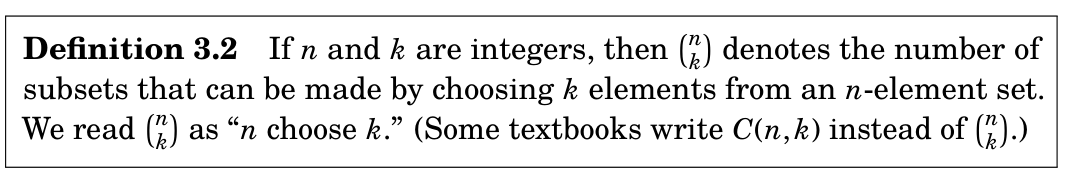
\includegraphics[width=0.9\textwidth]{images/definition03_02.png}
\end{figure}
\begin{figure}
   \centering
   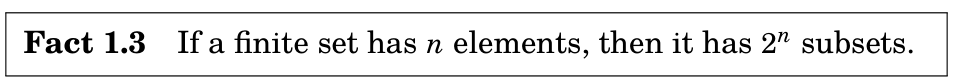
\includegraphics[width=0.9\textwidth]{images/fact01_03.png}
\end{figure}

\begin{prooflist}{7. Use the binomial theorem to show the following.}
    \item
        $$\sum\limits_{k=0}^n 3^k \binom{n}{k}=4^n$$
\item
    The binomial theorem asserts the following.
    $$
    (x+y)^n = \sum\limits_{k=0}^n \dbinom{n}{k} x^{n-k}y^k
    $$
\item Let $x=1, y=3$, then
    $$
    (1+3)^n = \sum\limits_{k=0}^n \dbinom{n}{k} 1^{n-k}3^k
    $$
    $$
    4^n = \sum\limits_{k=0}^n \dbinom{n}{k} 3^k
    $$
\end{prooflist}


\begin{prooflist}{8. Use Fact 3.5 (page 87) to derive Equation 3.3 (page 90).}
\item First let's expand out the right hand side, and get a common denominator.
    $$\dbinom{n}{k-1} =\dfrac{n!}{(k-1)!(n-k+1)!}$$
    $$=\dfrac{n!}{(k-1)!(n-k)!(n-k+1)} =\dfrac{kn!}{k(k-1)!(n-k)!(n-k+1)}$$

    $$\dbinom{n}{k}=\dfrac{n!}{k!(n-k)!}=
    \dfrac{n!}{k(k-1)!(n-k)!}=
    \dfrac{(n-k+1)n!}{(n-k+1)k(k-1)!(n-k)!}
    $$

    $$\dbinom{n}{k-1} + \dbinom{n}{k}=$$
    $$ \dfrac{kn!+(n-k+1)n!}{(n-k+1)k(k-1)!(n-k)!}=
    \dfrac{n!(k+n-k+1)}{(n-k+1)!k!}= $$
    $$ \dfrac{n!(n+1)}{(n-k+1)!k!}=
    \dfrac{(n+1)!}{(n-k+1)!k!}= \dbinom{n+1}{k}$$

\end{prooflist}
\begin{figure}
   \centering
   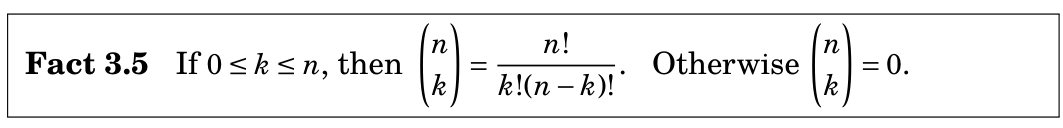
\includegraphics[width=0.9\textwidth]{images/fact03_05.png}
\end{figure}
\begin{figure}
   \centering
   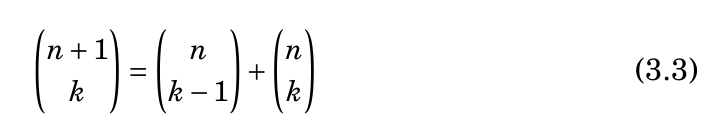
\includegraphics[width=0.9\textwidth]{images/equation03_03.png}
\end{figure}

\begin{prooflist}{9. Use the binomial theorem to show}
\item
    $$
    \dbinom{n}{0}
    - \dbinom{n}{1}
    + \dbinom{n}{2}
    - \dbinom{n}{3}
    + \dbinom{n}{4}
    \dots
    + (-1)^n\dbinom{n}{n} =0, \quad n>0.
    $$
\item The binomial theorem states
    $$(x+y)^n=\sum\limits_{i=0}^n\dbinom{n}{i}x^{n-i}y^i$$
    $$
    \dbinom{n}{0}
    - \dbinom{n}{1}
    + \dbinom{n}{2}
    - \dbinom{n}{3}
    + \dbinom{n}{4}
    \dots
    + (-1)^n\dbinom{n}{n}=(1+(-1))^n = 0^n = 0
    $$
\end{prooflist}

\begin{prooflist}{10. Show that the formula $k\dbinom{n}{k}=n\dbinom{n-1}{k-1}$
    is true for all integers $n, k$ with $0 \leq k \leq n$.}
\item Suppose $k\neq0$
    $$k\dbinom{n}{k}=n\dbinom{n-1}{k-1}$$
    $$k\dfrac{n!}{(n-k)!k!}=n\dfrac{(n-1)!}{(k-1)!(n-1-k+1)!}$$
    $$k\dfrac{n!}{(n-k)!k!}=\dfrac{n!}{(k-1)!(n-k)!}$$
    $$k\dfrac{n!}{(n-k)!k!}=\dfrac{n!}{(k-1)!(n-k)!}\cdot\dfrac{k}{k}$$
    $$k\dfrac{n!}{(n-k)!k!}=k\dfrac{n!}{(n-k)!k!}$$
\item Suppose $k=0$
    $$0\cdot\dbinom{n}{0}=n\dbinom{n-1}{-1}$$
    $$0\cdot\dbinom{n}{0}=n\cdot 0$$
    $$0=0$$
\end{prooflist}

\begin{prooflist}{11. Use the binomial theorem to show}
\item
    $$9^n=\sum\limits_{k=0}^{n} (-1)^k\dbinom{n}{k}10^{n-k}$$
\item The binomial theorem states
    $$(x+y)^n=\sum\limits_{i=0}^n\dbinom{n}{i}x^{n-i}y^i$$
\item let $x=-1, y=10$
    $$((-1)+10)^n=\sum\limits_{k=0}^{n} (-1)^k\dbinom{n}{k}10^{n-k}$$
\end{prooflist}

\begin{prooflist}{12. Show that
    $$
\dbinom{n}{k}
\dbinom{k}{m}=
\dbinom{n}{m}
\dbinom{n-m}{k-m}
$$}
\item
$$
\dbinom{n}{k}
\dbinom{k}{m}=
\dfrac{n!}{(n-k)!k!}
\dfrac{k!}{(m-k)!m!}=
\dfrac{n!}{(n-k)!(m-k)!m!}
$$
$$
\dbinom{n}{m}
\dbinom{n-m}{k-m}=
\dfrac{n!}{(n-m)!m!}\cdot
\dfrac{(n-m)!}{(k-m)!(n-m-k+m)!}=
$$
$$
\dfrac{n!}{m!}\cdot
\dfrac{1}{(k-m)!(n-k)!}=\dfrac{n!}{(n-k)!(m-k)!m!}
$$
\end{prooflist}

\begin{prooflist}{13. Show that}
    \item
$$
\dbinom{n}{3}=
\dbinom{2}{2} +
\dbinom{3}{2} +
\dbinom{4}{2} +
\dbinom{5}{2} +
\dots +
\dbinom{n-1}{2}
$$

\item Remember this equality:
    $$\dbinom{n+1}{k} = \dbinom{n}{k} + \dbinom{n}{k-1}$$

\item The binomial theorem states
    $$(x+y)^n=\sum\limits_{i=0}^n\dbinom{n}{i}x^{n-i}y^i$$
\item

\item Suppose $k=3$
$$
\dbinom{n}{3}=
\dbinom{n-1}{2} +
\dbinom{n-1}{3}
$$
$$
\dbinom{n-1}{3} =
\dbinom{n-2}{2} +
\dbinom{n-2}{3}
$$
$$
\dbinom{n-2}{3} =
\dbinom{n-3}{2} +
\dbinom{n-3}{3}
$$
$$
\dots
$$
\begin{figure}
   \centering
   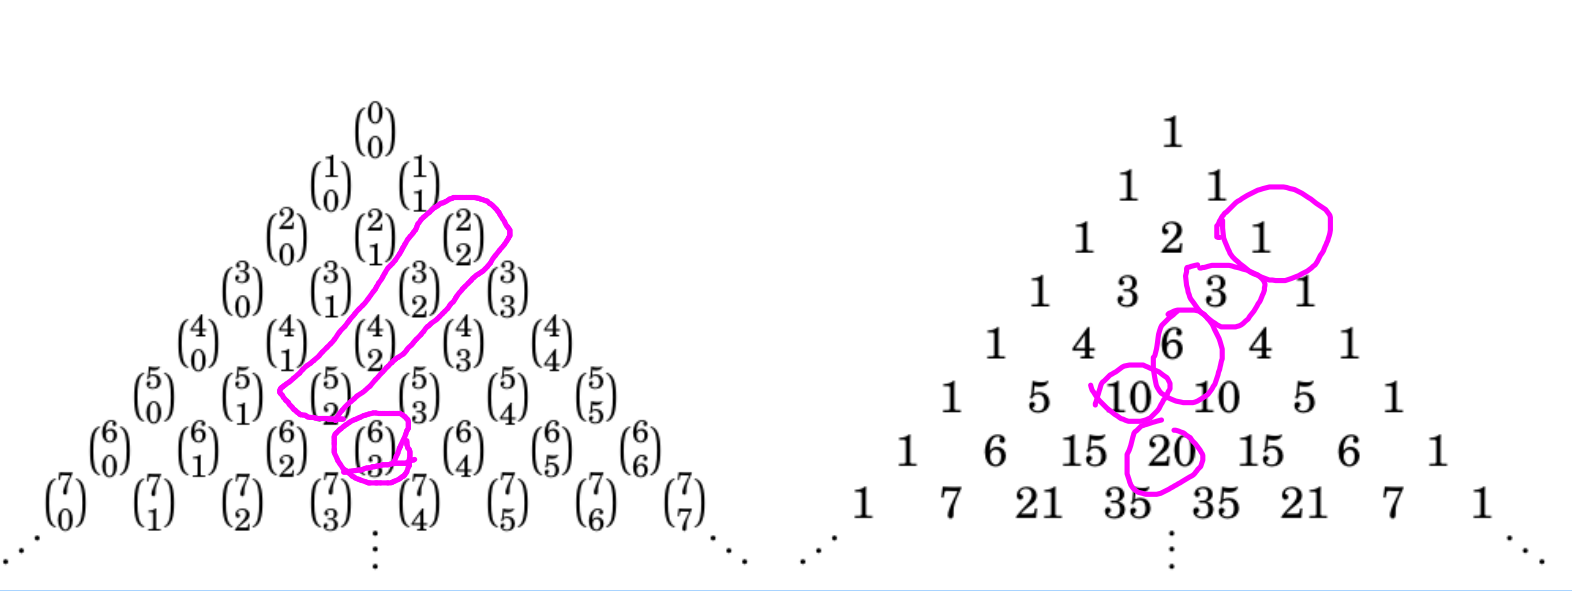
\includegraphics[width=0.7\textwidth]{images/pascals-triangle.png}
\end{figure}

\end{prooflist}

% 14. The first five rows of Pascal’s triangle appear in the digits of powers of 11: 110 = 1,
% 111 = 11, 112 = 121, 113 = 1331 and 114 = 14641. Why is this so? Why does the
% pattern not continue with 115?

\end{document}
